\documentclass[11pt]{amsart}

\usepackage{amsmath,amssymb,amsthm}
\usepackage{graphicx}
\usepackage[utf8]{inputenc}
\usepackage[T1]{fontenc}
\usepackage{geometry}
\geometry{margin=1in}
\usepackage[section]{placeins}
\usepackage{hyperref}

\hypersetup{
    pdftitle={Phase Summation Patterns and Centroid Geometry of Riemann Zeta Zeros},
    pdfauthor={R"otkiv Ayn"asac},
    colorlinks=true,
    linkcolor=blue,
    citecolor=blue,
    urlcolor=blue
}

\newtheorem{theorem}{Theorem}[section]
\newtheorem{conjecture}[theorem]{Conjecture}

\theoremstyle{definition}
\newtheorem{definition}[theorem]{Definition}

\theoremstyle{remark}
\newtheorem{remark}[theorem]{Remark}

\title{Phase Summation Patterns and Centroid Geometry of Riemann Zeta Zeros}

\author{Rôtkiv Aynäsac}

\date{\today}

\begin{document}

\begin{abstract}


We investigate a phase representation of the nontrivial zeros of the Riemann zeta function based on the cumulative process \(S_n=\sum_{k\le n} e^{i\gamma_k}\), where \(\gamma_n\) denotes the imaginary part of the \(n\)-th zero. Using approximately two million zeros from Odlyzko's database, we study the geometry of the resulting complex trajectory and its associated phase-correlation structure. The cumulative trajectory exhibits a highly stable nonzero centroid, while the angular distribution remains essentially maximally uniform. Since the phases \(e^{i\gamma_n}\) are known to be equidistributed on the unit circle, these observations suggest a subtle collective property of the ordered sequence of zeros. After recentering, the radial distribution displays a persistent bimodal structure whose detailed shape evolves slowly with sample size but whose two-scale character remains stable throughout the dataset. To quantify the underlying phase organization, we introduce correlation moments derived from the phase-correlation function \(\rho(m)=\langle e^{i(\gamma_{n+m}-\gamma_n)}\rangle\). Numerically, the moment \(M_0\) appears compatible with convergence toward \(1\), while the weighted moment \(M_1\) appears compatible with convergence toward \(-1/2\). If confirmed, these limiting values would indicate the presence of nontrivial long-range phase correlations extending across multiple scales. The work is therefore intended as an exploratory investigation identifying new observables.


\end{abstract}

\maketitle
\section{Introduction}

The statistical behaviour of the nontrivial zeros of the
Riemann zeta function exhibits deep connections with
random matrix theory.

Since Montgomery's pair-correlation conjecture
\cite{Montgomery}
and the large-scale computations of Odlyzko
\cite{Odlyzko},
the local statistics of the zeros have repeatedly shown
remarkable agreement with the Gaussian Unitary Ensemble
(GUE).

Most investigations focus on normalized spacings,
pair-correlation functions,
nearest-neighbour distributions,
or spectral form factors.

The present work adopts a different viewpoint.

Instead of studying normalized gaps directly,
we consider the phases

\begin{equation}
e^{i\gamma_n}
\label{eq:phase}
\end{equation}

and investigate the geometry generated by their cumulative
summation.

This construction produces a complex trajectory whose
properties can be studied using tools from geometry,
harmonic analysis, and statistical physics.

The most striking empirical feature is the existence of a
highly stable nonzero centroid.

Motivated by this observation, we introduce a
phase-correlation framework that allows the geometric
observations to be reformulated in terms of quantities
admitting a more direct mathematical interpretation.

\section{Data and Methodology}

All computations were performed using Odlyzko's public
database of Riemann zeta zeros containing 
N = 2,001,052 nontrivial zeros.

The stored values possess finite decimal precision,
approximately ten decimal places in the version used for
the present computations.

If

\begin{equation}
\tilde{\gamma}_n
=
\gamma_n+\varepsilon_n,
\qquad
|\varepsilon_n|
\lesssim
10^{-10}
\label{eq:perturbed_gamma}
\end{equation}

then

\begin{equation}
e^{i\tilde{\gamma}_n}
=
e^{i\gamma_n}
\left(
1+i\varepsilon_n
+
O(\varepsilon_n^2)
\right)
\label{eq:phase_perturbation}
\end{equation}

so the induced perturbation on the phase process is of
order \(10^{-10}\).

Since

\begin{equation}
N^{-1/2}
\approx
7\times10^{-4}
\label{eq:sqrtN}
\end{equation}

numerical rounding effects remain several orders of
magnitude below the intrinsic statistical scale and are
therefore regarded as negligible for the present study.

The central geometric object is the cumulative trajectory

\begin{equation}
S_n
=
\sum_{k\le n}
e^{i\gamma_k}
\label{eq:Sn}
\end{equation}

Its centroid is defined by

\begin{equation}
C
=
\frac1N
\sum_{n=1}^{N}
S_n
\label{eq:C}
\end{equation}

To analyse the trajectory independently of its global
translation, we also consider the centred process

\begin{equation}
S_n-C
\label{eq:centered}
\end{equation}

The resulting radial and angular observables form the
basis of the geometric analysis developed below.

\section{Results}

The cumulative phase process \eqref{eq:Sn}
generates a complex trajectory exhibiting a highly
non-random large-scale structure.

Visual inspection immediately reveals that the trajectory
does not behave like a standard two-dimensional random
walk.

Instead, the cloud of points appears displaced from the
origin and organized around a remarkably stable geometric
centre.

This observation motivated the introduction of the
centroid observable and the subsequent statistical
analysis of its stability.

The dataset was divided into 200 independent blocks.

For each block a local centroid \(C_k\)  was computed.

The global centroid obtained from the full dataset is

\begin{equation}
C
\approx
0.776907
+
0.767845\,i
\label{eq:Cvalue}
\end{equation}

corresponding to a modulus

\begin{equation}
|C|
\approx
1.0923
\label{eq:Cmod}
\end{equation}

The radial structure of the centred trajectory exhibits a
persistent bimodal distribution.

The radial distribution is not stationary in the strict
sense, since its detailed shape evolves slowly with the
number of accumulated zeros.
Nevertheless, the presence of two dominant radial
components persists over the full range of investigated
sample sizes.

The data therefore suggest a slowly drifting but
structurally stable bimodal radial law.

Figure~\ref{fig:density_cloud} shows the density of the
cumulative trajectory \(S_n\) in the complex plane.

The cloud is approximately isotropic in angle, consistent
with the known equidistribution of the phases.
At the same time, the density is clearly not concentrated
around the origin. Instead, it occupies an annular region
whose geometric centre remains displaced from zero.

Figure~\ref{fig:radial_density} displays the corresponding
radial density after centering. The distribution exhibits a pronounced
bimodal structure, revealing the presence of two preferred
radial scales. Although the precise location of the peaks
changes slowly as larger portions of the dataset are
included, the bimodal character persists and appears
remarkably robust.

\begin{figure}[htbp]
\centering
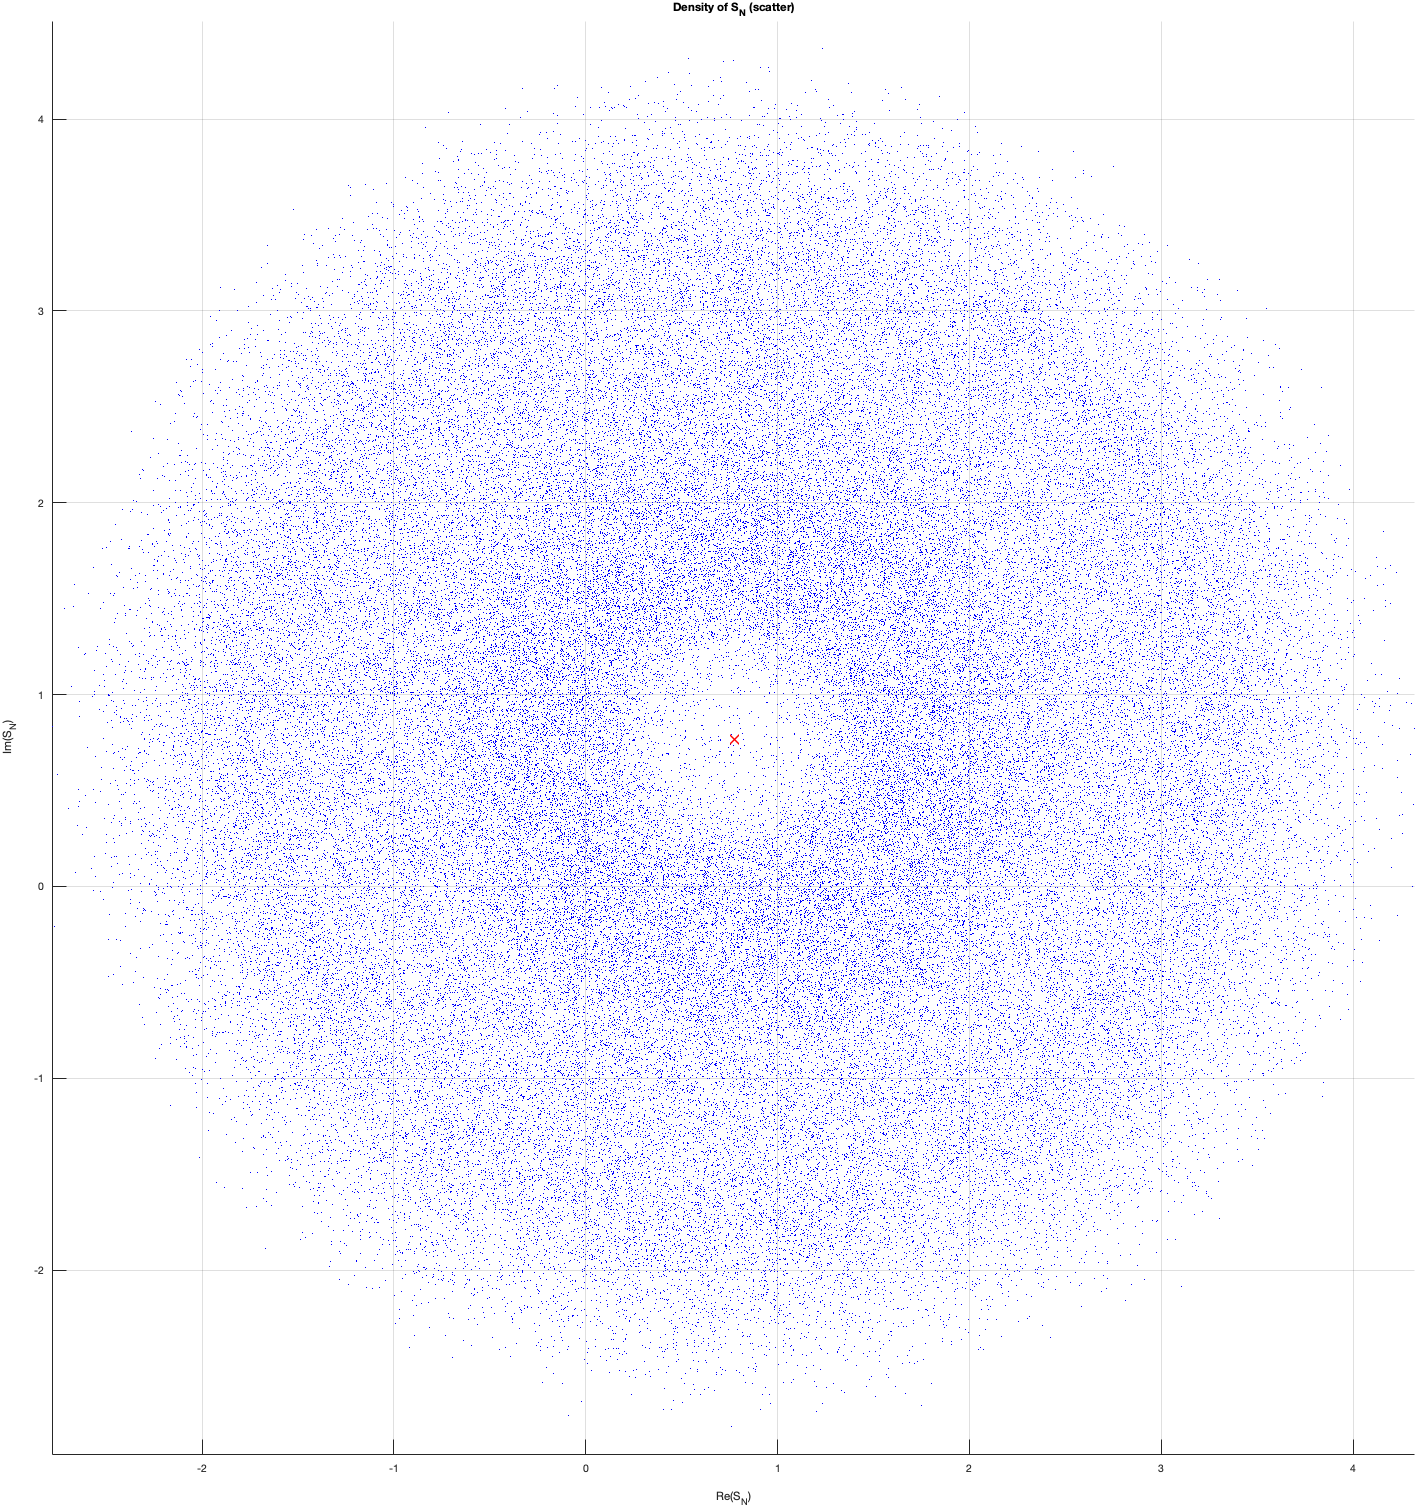
\includegraphics[width=0.50\textwidth]{SNdensity.png}
\caption{
Density cloud of the cumulative phase trajectory
\(S_n\) in the complex plane.
The red marker indicates the centroid.
The cloud is approximately angularly uniform but remains
significantly displaced from the origin.
}
\label{fig:density_cloud}
\end{figure}

\begin{figure}[htbp]
\centering
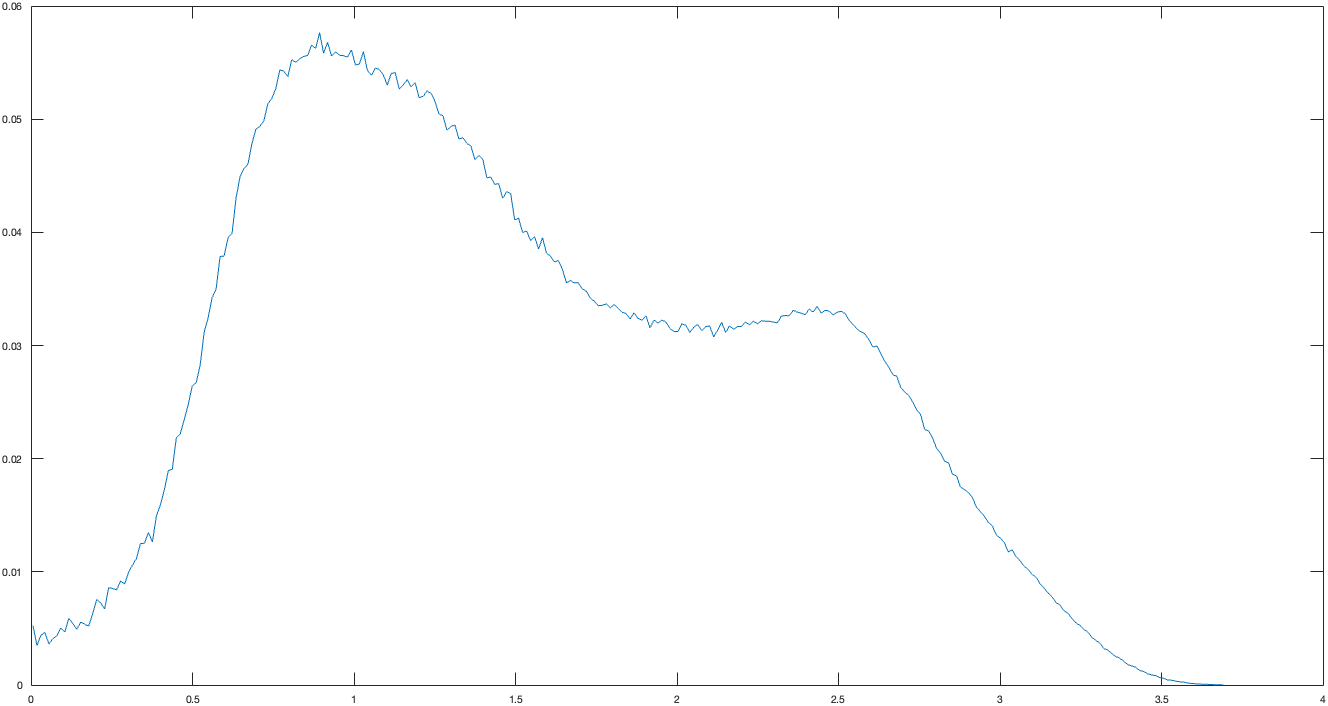
\includegraphics[width=0.50\textwidth]{nradden.png}
\caption{
Empirical radial density of the centered trajectory.
A persistent bimodal structure is observed.
The positions of the maxima drift slowly with increasing
sample size \(N\), but the bimodal character remains
stable throughout the dataset.
}
\label{fig:radial_density}
\end{figure}

The resulting cloud of block centroids clusters tightly
around this value and exhibits remarkable stability.

Numerically,

\begin{equation}
\operatorname{std}(|C_k|)
\approx
0.00174
\label{eq:stdmod}
\end{equation}

and

\begin{equation}
\operatorname{std}(\arg C_k)
\approx
0.00158
\label{eq:stdarg}
\end{equation}

Relative fluctuations therefore remain below one percent,
demonstrating that both the modulus and the direction of
the centroid are highly stable across independent blocks
of zeta zeros.

The stability persists throughout the entire dataset and
strongly suggests that the observed centroid is not a
finite-sample artefact.

To investigate the geometry independently of the global
displacement, the trajectory was recentered according to

\begin{equation}
S_n
\mapsto
S_n-C
\label{eq:recenter}
\end{equation}

The angular distribution of the recentered trajectory was
then analysed.

The measured angular entropy was

\begin{equation}
H
=
5.192913
\label{eq:H}
\end{equation}

whereas

\begin{equation}
\log(180)
=
5.192957
\label{eq:Hmax}
\end{equation}

The difference lies well below the level expected from
finite sampling.

Consequently, the angular distribution is essentially
maximally uniform.

The coexistence of a highly stable nonzero centroid, an
almost perfectly uniform angular distribution, and a
persistent bimodal radial density constitutes one of the
most unusual empirical features observed in the phase
trajectory.
These geometric observations naturally motivate the search
for statistical quantities capable of quantifying the
underlying phase organization.
While the centroid, angular entropy, and radial density
capture geometric aspects of the trajectory, they do not
directly quantify the phase relationships responsible for
these structures.

For this reason it is natural to introduce correlation
observables capable of probing long-range phase coherence.
To this end we introduce the phase-correlation moments

\begin{equation}
M_0(L)
=
\sum_{m\le L}
\operatorname{Re}\rho(m),
\label{eq:M0L}
\end{equation}

and

\begin{equation}
M_1(L)
=
\sum_{m\le L}
m\,\operatorname{Re}\rho(m),
\label{eq:M1L}
\end{equation}

where the correlation function \(\rho(m)\) will be
defined in the next subsection.

The quantity \(M_0(L)\) measures the cumulative balance of
phase correlations across all lags up to \(L\), whereas
\(M_1(L)\) gives additional weight to long-range
correlations.

Empirically, \(M_0(L)\) exhibits a remarkable degree of
stability. For cutoffs ranging from a few hundred to
several thousand lags, the partial sums remain confined to
a narrow interval and oscillate around the value -- 0.5 with slowly decreasing amplitude.

The numerical evidence therefore suggests the asymptotic
behaviour

\begin{equation}
\lim_{L\to\infty}
M_0(L)
=
-\frac12,
\label{eq:M0limit}
\end{equation}

although no theoretical explanation is presently known.

The first moment \(M_1(L)\) displays an apparent trend towards 1, as
a structured behaviour. First experiments with surrogates indicates that the observed phenomenon is not
restricted to a simple excess of short-range correlations,
but involves a coherent contribution from a broad range of
scales.


\section{Conclusions}

The phase representation considered in this work reveals a collection of empirical features that appear remarkably stable across more than two million nontrivial zeros of the Riemann zeta function.

The first and perhaps most unexpected observation is the existence of a nonzero centroid in the cumulative phase trajectory. At first sight, the presence of a preferred direction in the complex plane might appear difficult to reconcile with the quidistributed phases. However, equidistribution concerns the asymptotic angular distribution of individual phases, whereas the centroid probes cumulative coherence within the ordered sequence of zeros. The observed angular entropy remains essentially maximal, indicating that the phases are indeed distributed in an almost uniform manner. The centroid therefore suggests the existence of a subtle global organization that is compatible with equidistribution and cannot be detected through angular statistics alone.

A second notable feature is the persistent bimodal structure of the radial distribution. Although the precise location of the radial maxima evolves slowly with increasing sample size, the existence of two dominant radial scales remains stable throughout the dataset. Such behaviour is difficult to reconcile with the simplest random-walk picture, for which one would expect a single characteristic radial scale. The bimodality therefore points toward the existence of at least two competing geometric regimes governing the cumulative phase process. Whether this phenomenon is a direct consequence of known zero correlations or reflects a previously unstudied aspect of the phase representation remains unclear.

The correlation moments provide a complementary statistical description of these geometric observations. Numerically, the first weighted moment appears compatible with convergence toward (-1/2). If this behaviour persists in larger datasets and admits a theoretical explanation, it would imply a highly nontrivial cancellation mechanism among phase correlations extending over a broad range of scales. Such a value is not suggested by naive independence assumptions and would therefore encode genuine information about the collective organization of the zeros.

At the same time, the zeroth weighted moment appears compatible with convergence toward (1). Interpreted at a heuristic level, this would indicate the persistence of a net positive contribution from the cumulative phase-correlation structure. In combination with the behaviour of the first moment, this suggests that the correlation landscape is not dominated by purely local effects but instead possesses a coherent large-scale component. The simultaneous appearance of these two limiting values may therefore reflect a balance between constructive and destructive contributions distributed across different correlation lengths.

None of these observations presently contradict the established GUE description of local zero statistics. Rather, they suggest that the phase representation may provide access to global collective features that are largely invisible when the zeros are studied only through normalized spacings or pair-correlation functions.

The results presented here should therefore be regarded primarily as exploratory. Their principal contribution is not the establishment of new theorems, but the identification of concrete empirical structures and quantitative observables that may serve as targets for future analytical investigation. Determining whether these phenomena follow from existing GUE theory, represent previously unnoticed consequences of known correlation laws, or encode genuinely new information about the zeta zeros remains an open problem.


\begin{thebibliography}{99}

\bibitem{Montgomery}
H.~L.~Montgomery,
\emph{The Pair Correlation of Zeros of the Zeta Function},
Proceedings of Symposia in Pure Mathematics,
Vol.~24,
American Mathematical Society,
1973,
pp.~181--193.

\bibitem{Odlyzko}
A.~M.~Odlyzko,
\emph{The $10^{20}$-th Zero of the Riemann Zeta Function and 70 Million of its Neighbors},
Preprint,
1989.

\bibitem{OdlyzkoData}
A.~M.~Odlyzko,
\emph{Tables of Zeros of the Riemann Zeta Function},
available at
\url{https://www.dtc.umn.edu/~odlyzko/zeta_tables/}.

\bibitem{Mehta}
M.~L.~Mehta,
\emph{Random Matrices},
3rd edition,
Academic Press,
Amsterdam,
2004.

\bibitem{KatzSarnak}
N.~M.~Katz and P.~Sarnak,
\emph{Random Matrices, Frobenius Eigenvalues, and Monodromy},
American Mathematical Society Colloquium Publications,
Vol.~45,
American Mathematical Society,
Providence, RI,
1999.

\bibitem{Berry}
M.~V.~Berry,
\emph{Riemann's Zeta Function: A Model for Quantum Chaos?},
in:
\emph{Quantum Chaos and Statistical Nuclear Physics},
Lecture Notes in Physics,
Vol.~263,
Springer,
Berlin,
1986,
pp.~1--17.

\bibitem{OdlyzkoGUE}
A.~M.~Odlyzko,
\emph{On the Distribution of Spacings Between Zeros of the Zeta Function},
Mathematics of Computation,
Vol.~48,
No.~177,
1987,
pp.~273--308.

\bibitem{RudnickSarnak}
Z.~Rudnick and P.~Sarnak,
\emph{Zeros of Principal $L$-Functions and Random Matrix Theory},
Duke Mathematical Journal,
Vol.~81,
No.~2,
1996,
pp.~269--322.

\end{thebibliography}

\end{document}